\documentclass[manuscript]{aastex6}

% to-do list
% ----------
% - Add references and uncertainties to Table 1

% style notes
% -----------
% - This file generates by Makefile; don't be typing ``pdflatex'' or some bullshit.
% - Line break between sentences to make the git diffs readable.
% - Use \, as a multiply operator.
% - Reserve () for function arguments; use [] or {} for outer shit.
% - Use \sectionname not Section, \figname not Figure, \documentname not Article or Paper or paper.

\include{gitstuff}
% ----------------------------------- %
% start of AASTeX mods by DWH and DFM %
% ----------------------------------- %

\setlength{\voffset}{0in}
\setlength{\hoffset}{0in}
\setlength{\textwidth}{6in}
\setlength{\textheight}{9in}
\setlength{\headheight}{0ex}
\setlength{\headsep}{\baselinestretch\baselineskip} % this is 2 lines in ``manuscript''
\setlength{\footnotesep}{0in}
\setlength{\topmargin}{-\headsep}
\setlength{\oddsidemargin}{0.25in}
\setlength{\evensidemargin}{0.25in}

\linespread{0.54} % close to 10/13 spacing in ``manuscript''
\setlength{\parindent}{0.54\baselineskip}
\hypersetup{colorlinks = false}
\makeatletter % you know you are living your life wrong when you need to do this
\long\def\frontmatter@title@above{
\vspace*{-\headsep}\vspace*{\headheight}
\noindent\footnotesize
{\noindent\footnotesize\textsc{\@journalinfo}}\par
{\noindent\scriptsize Preprint typeset using \LaTeX\ style AASTeX6
with modifications by DWH and DFM.
}\par\vspace*{-\baselineskip}\vspace*{0.625in}
}%
\long\def\frontmatter@abstractheading{%
\makeaffils
  \vspace*{-\baselineskip}\vspace*{1.5pt}
  \vspace*{0.13189in}
 \begingroup
  \centering
  \abstractname
  \vskip 1mm
  \par
 \endgroup
 \everypar{\rightskip=0.0in\leftskip=\rightskip}\par
}%
\def\frontmatter@keys@format{\vspace*{0.5mm}%
  \settowidth{\keys@width}{\normalsize\@keys@name}%
  \rightskip=0.0in\leftskip=\rightskip\parindent=0pt%
    \hangindent=\keys@width\hangafter=1\normalsize\raggedright}%
\def\twodigits#1{\ifnum#1<10 0\fi\the#1}
\def\mydate{\leavevmode\hbox{\the\year-\twodigits\month-\twodigits\day}}
\makeatother
\renewcommand{\today}{\mydate}

% Section spacing:
\makeatletter
\let\origsection\section
\renewcommand\section{\@ifstar{\starsection}{\nostarsection}}
\newcommand\nostarsection[1]{\sectionprelude\origsection{#1}}
\newcommand\starsection[1]{\sectionprelude\origsection*{#1}}
\newcommand\sectionprelude{\vspace{1em}}
\let\origsubsection\subsection
\renewcommand\subsection{\@ifstar{\starsubsection}{\nostarsubsection}}
\newcommand\nostarsubsection[1]{\subsectionprelude\origsubsection{#1}}
\newcommand\starsubsection[1]{\subsectionprelude\origsubsection*{#1}}
\newcommand\subsectionprelude{\vspace{1em}}
\makeatother

\widowpenalty=10000
\clubpenalty=10000

\sloppy\sloppypar

% ------------------ %
% end of AASTeX mods %
% ------------------ %


% packages
\definecolor{cbblue}{HTML}{3182bd}
\usepackage{microtype}  % ALWAYS!
\usepackage{amsmath,amssymb,natbib}
\usepackage[flushleft]{threeparttable}
\hypersetup{backref,breaklinks,colorlinks,urlcolor=cbblue,linkcolor=cbblue,citecolor=black}
\graphicspath{{figures/}}

% define macros for text
\newcommand{\project}[1]{\textsl{#1}}
\newcommand{\acronym}[1]{{\small{#1}}}
\newcommand{\gaia}{\project{Gaia}}
\newcommand{\rave}{\project{\acronym{RAVE}}}
\newcommand{\apogee}{\project{\acronym{APOGEE}}}
\newcommand{\tmass}{\project{\acronym{2MASS}}}
\newcommand{\documentname}{Article}
\newcommand{\sectionname}{Section}
\newcommand{\figname}{Figure}
\newcommand{\eqname}{Equation}
\newcommand{\dr}{\acronym{DR1}}
\newcommand{\tgas}{\acronym{TGAS}}
\newcommand{\etal}{\textit{et al}.}
\newcommand*\elem[1]{\ensuremath{\mathrm{#1}}}
\newcommand*\elemH[1]{\ensuremath{[\mathrm{#1}/\elem{H}]}}
\newcommand*{\feh}{\ensuremath{\elemH{Fe}}}
\newcommand{\sunanalog}{\text{HD 240429}}
\newcommand{\bizarreone}{\text{HD 240430}}



% define macros for math
\newcommand{\given}{\,|\,}
\newcommand{\normal}{{\mathcal{N}}}
\newcommand{\dd}{\mathrm{d}}
\newcommand{\transp}[1]{{#1}^{\!\mathsf{T}}}
\newcommand{\inv}[1]{{#1}^{-1}}
\newcommand{\bs}[1]{\boldsymbol{#1}}
\newcommand{\vperp}{\bs{v}^\perp}
\newcommand{\propm}{\bs{\mu}}
\newcommand{\mat}[1]{\mathbf{#1}}
\renewcommand{\vec}[1]{\bs{#1}}
\newcommand{\kms}{\ensuremath{\rm km~s^{-1}}}
\newcommand{\msun}{{\rm M}_\odot}
\newcommand{\pc}{{\rm pc}}
\newcommand{\data}{\mathrm{data}}
\newcommand{\snr}{[S/N]_\varpi}
\newcommand{\eye}{\mathbb{I}}
\newcommand{\absdvtan}{\ensuremath{|\Delta\vec v_\mathrm{t}|}}
\newcommand{\estimates}{\ensuremath{\{\hat{\varpi_i},\hat{\mu_{\alpha,i}},\hat{\mu_{\delta,i}},\hat{v_{r,i}}\}}}

\newcommand{\todo}[1]{{\color{blue}TODO:#1}}

\renewcommand\tablename{Table}

\begin{document}\sloppy\sloppypar\raggedbottom\frenchspacing % trust me

\title{A pair of co-moving, Sun-like stars with different chemical abundances:\\
       a possible signature of copious rocky accretion (needs work)}

\author{
  Semyeong Oh\altaffilmark{\pu,\lead},
  APW, JMB, KH, NL, DWH, DNS
}

% Affiliations
\newcommand{\pu}{1}
\newcommand{\lead}{2}
\newcommand{\ccpp}{3}
\newcommand{\mpia}{4}
\newcommand{\cca}{5}

\altaffiltext{\pu}{Department of Astrophysical Sciences,
                   Princeton University, Princeton, NJ 08544, USA}
\altaffiltext{\lead}{To whom correspondence should be addressed:
                     \texttt{semyeong@astro.princeton.edu}}
\altaffiltext{\ccpp}{Center for Cosmology and Particle Physics,
                     Department of Physics,
                     New York University, 4 Washington Place,
                     New York, NY 10003, USA}
\altaffiltext{\mpia}{Max-Planck-Institut f\"ur Astronomie,
                     K\"onigstuhl 17, D-69117 Heidelberg, Germany}
\altaffiltext{\cca}{Center for Computational Astrophysics, 162 5th Ave, New York, NY 10003, USA}


\begin{abstract}
  We report and discuss the discovery of a co-moving pair of bright solar-type
  stars, \sunanalog\ and \bizarreone\, with significant differences in their chemical
  abundance patterns.
  The two stars are co-spatial ($|\Delta \bs{x}| < XX~\pc$) at a distance of
  $r\approx 100~\pc$ with nearly identical three-dimensional velocities
  ($|\Delta \bs{v}| < XX~\kms$ with 95\% confidence), as inferred from \gaia\
  \tgas\ proper motions and high resolution radial velocity measurements.
  Both stars are young with ages $\approx$$500~{\rm Myr}$ as estimated from
  their lithium abundances, favoring the idea that they were born together and
  are or were recently a bound, wide binary system.
  However, the metallicities and chemical abundances of refractory
  elements in the two stars are very different, challenging this simple picture.
  In order to reconcile the seemingly contradictory observations,
  we consider scenarios in which the pair is unrelated despite
  its current spatial and kinematic configuration, and
  those in which the pair formed together but may now have different chemistry.
  In the latter, we consider the possibility that the more metal-rich of the two,
  \bizarreone, accreted $\approx$10's of Earth masses of protoplanetary, rocky material,
  selectively enhancing the refractory elements.
  Direct-imaging and precision radial velocity follow-up to study the existence
  or properties of planetary systems around these stars would help distinguish
  these scenarios.
\end{abstract}

\section{Introduction} % (fold)
\label{sec:introduction}

% section introduction (end)

\section{Data}
\label{sec:data}

Though previously recognized as a visual double star system
(\citealt{2001AJ....122.3466M}), \sunanalog\ and \bizarreone\ were identified as a
candidate co-moving star pair in our recent search for co-moving stars using the
proper motions and parallaxes from the \tgas catalog, a component of \gaia\ \dr\
(the astrometric measurements are listed in \tablename~\ref{tab:t2}).
We refer the readers to this previous work (\citealt{2016arXiv161202440O}) for a
full explanation of the methodology behind this search and only briefly describe
the method here.
For a given pair, we compute a marginalized likelihood ratio between the
hypotheses (1) that a given pair of stars share the same 3D velocity vector, and
(2) that they have independent 3D velocity vectors, both given only observations
of two components of the velocities (proper motions).
We then select a sample of high-confidence co-moving star pairs by making a
conservative cut on this likelihood ratio.
In the resulting catalog of co-moving pairs (\citealt{2016arXiv161202440O}),
the pair presented in this paper was assigned a group id of 1199,
and the marginalized likelihood ratio (Bayes factor)
between the two hypotheses is $\ln{\mathcal{L}_1/\mathcal{L}_2} = 8.52$,
well above the adopted cut value of 6.
We have checked that we do not find any possible additional co-moving companions
by lowering the likelihood ratio cut for the stars around this pair.

In a separate effort to study detailed chemical abundances of
potential planet-hosting stars, \citet{2016ApJS..225...32B}
obtained high resolution spectroscopy for both \sunanalog\ and \bizarreone.
\todo{from where? mention briefly Keck HIRES}
The resulting measurements from this effort include abundances measured for 15
chemical species (C, N, O, Na, Mg, Al, Si, Ca, Ti, V, Cr, Mn, Fe, Ni, Y) as
well as high precision radial velocities.
Other stellar parameters derived from these spectra are included in
\tablename~\ref{tab:t2}.

Combining these precise radial velocities with the \gaia\ astrometry, we can
compare differences between the inferred 6D phase-space properties for the
two stars.
We start by generating posterior samples over the Heliocentric distance, $r$,
tangential velocities, $(v_\alpha, v_\delta)$, and radial velocity, $\hat{v}_r$,
given the observed parallax, $\pi$, and proper motion components,
$(\mu_{\alpha^*}, \mu_\delta)$, and radial velocity, $v_r$.
By defining the vectors
% SMOH: I understand you meant hat v_r as the latent true radial velocity but
% personally think a) it can confuse some people that there are hat quantities
% with no-hat quantities for hat-y vector and thus b) it'd be better to use hat
% quantities for observed variables and no-hat for latent true ones.
% SMOH: v_r is missing in the LHS of eq(3)
\begin{eqnarray}
  \vec{y} &=&
      \transp{\left(
        \begin{array}{c@{\hspace{1em}} c@{\hspace{1em}} c@{\hspace{1em}} c}
          \pi &
          \mu_{\alpha^*} &
          \mu_\delta &
          v_r
        \end{array}
      \right)}\\
  \hat{\vec{y}} &=&
      \transp{\left(
        \begin{array}{c@{\hspace{1em}} c@{\hspace{1em}} c@{\hspace{1em}} c}
          r^{-1} &
          r^{-1}\,v_\alpha &
          r^{-1}\,v_\delta &
          \hat{v}_r
        \end{array}
      \right)}
\end{eqnarray}
and by considering the covariance matrix $\mat{C}$ between the observed
quantities (provided by \tgas\ and extended to include the uncorrelated radial
velocity uncertainty), the likelihood can be written
\begin{eqnarray}
p(\pi, \mu_{\alpha^*}, \mu_\delta \given r, v_\alpha, v_\delta) &=&
  \left[\det\left(\frac{\mat{C}^{-1}}{2\pi}\right)\right]^{1/2} \,
    \exp \left[ -\frac{1}{2} \transp{\left(\vec{y} - \hat{\vec{y}} \right)} \,
    \mat{C}^{-1} \,
    \left(\vec{y} - \hat{\vec{y}} \right) \right] \label{eq:likefn} \quad .
\end{eqnarray}
We adopt a uniform space density prior for the distance and an isotropic
Gaussian for any velocity component, $v$, with a dispersion $\sigma_v=25~\kms$
\begin{eqnarray}
p(r) &=&
  \begin{cases}
    \frac{3}{r_{\rm lim}^3} \, r^2 & \text{if } 0 < r < r_{\rm lim}\\
    0              & \text{otherwise}
  \end{cases}\\
p(v) &=& \frac{1}{\sqrt{2\pi}\,\sigma_v} \,
  \exp\left[-\frac{1}{2} \, \frac{v^2}{\sigma_v^2} \right] \quad .
\end{eqnarray}
For each of the two stars, we use \project{emcee}
(\citealt{Foreman-Mackey:2013}) to generate posterior samples in $(r, v_\alpha,
v_\delta, \hat{v}_r)$ by running 64 walkers for 4608 steps and discarding the
first 512 steps as the burn-in period.
For each sample, we convert the heliocentric phase-space coordinates into
Galactocentric coordinates assuming the Sun's position and velocity are $x_\odot
= (-8.3, 0, 0)~{\rm kpc}$ and $v_\odot = (10, 244, 7.17)~\kms$ (\citealt{bovy,
etc.}).
\figurename~\ref{fig:dxdv} shows differences in posterior samples converted to
Galactocentric phase-space coordinates for the two stars.
In all components, the pair is consistent with being co-moving and close in
separation; the sky-projected separation of the two stars is $\approx$$0.01~\pc$
but the median 3-space separation is $\approx$$0.6~\pc$.

\begin{figure}[htbp]
  \begin{center}
    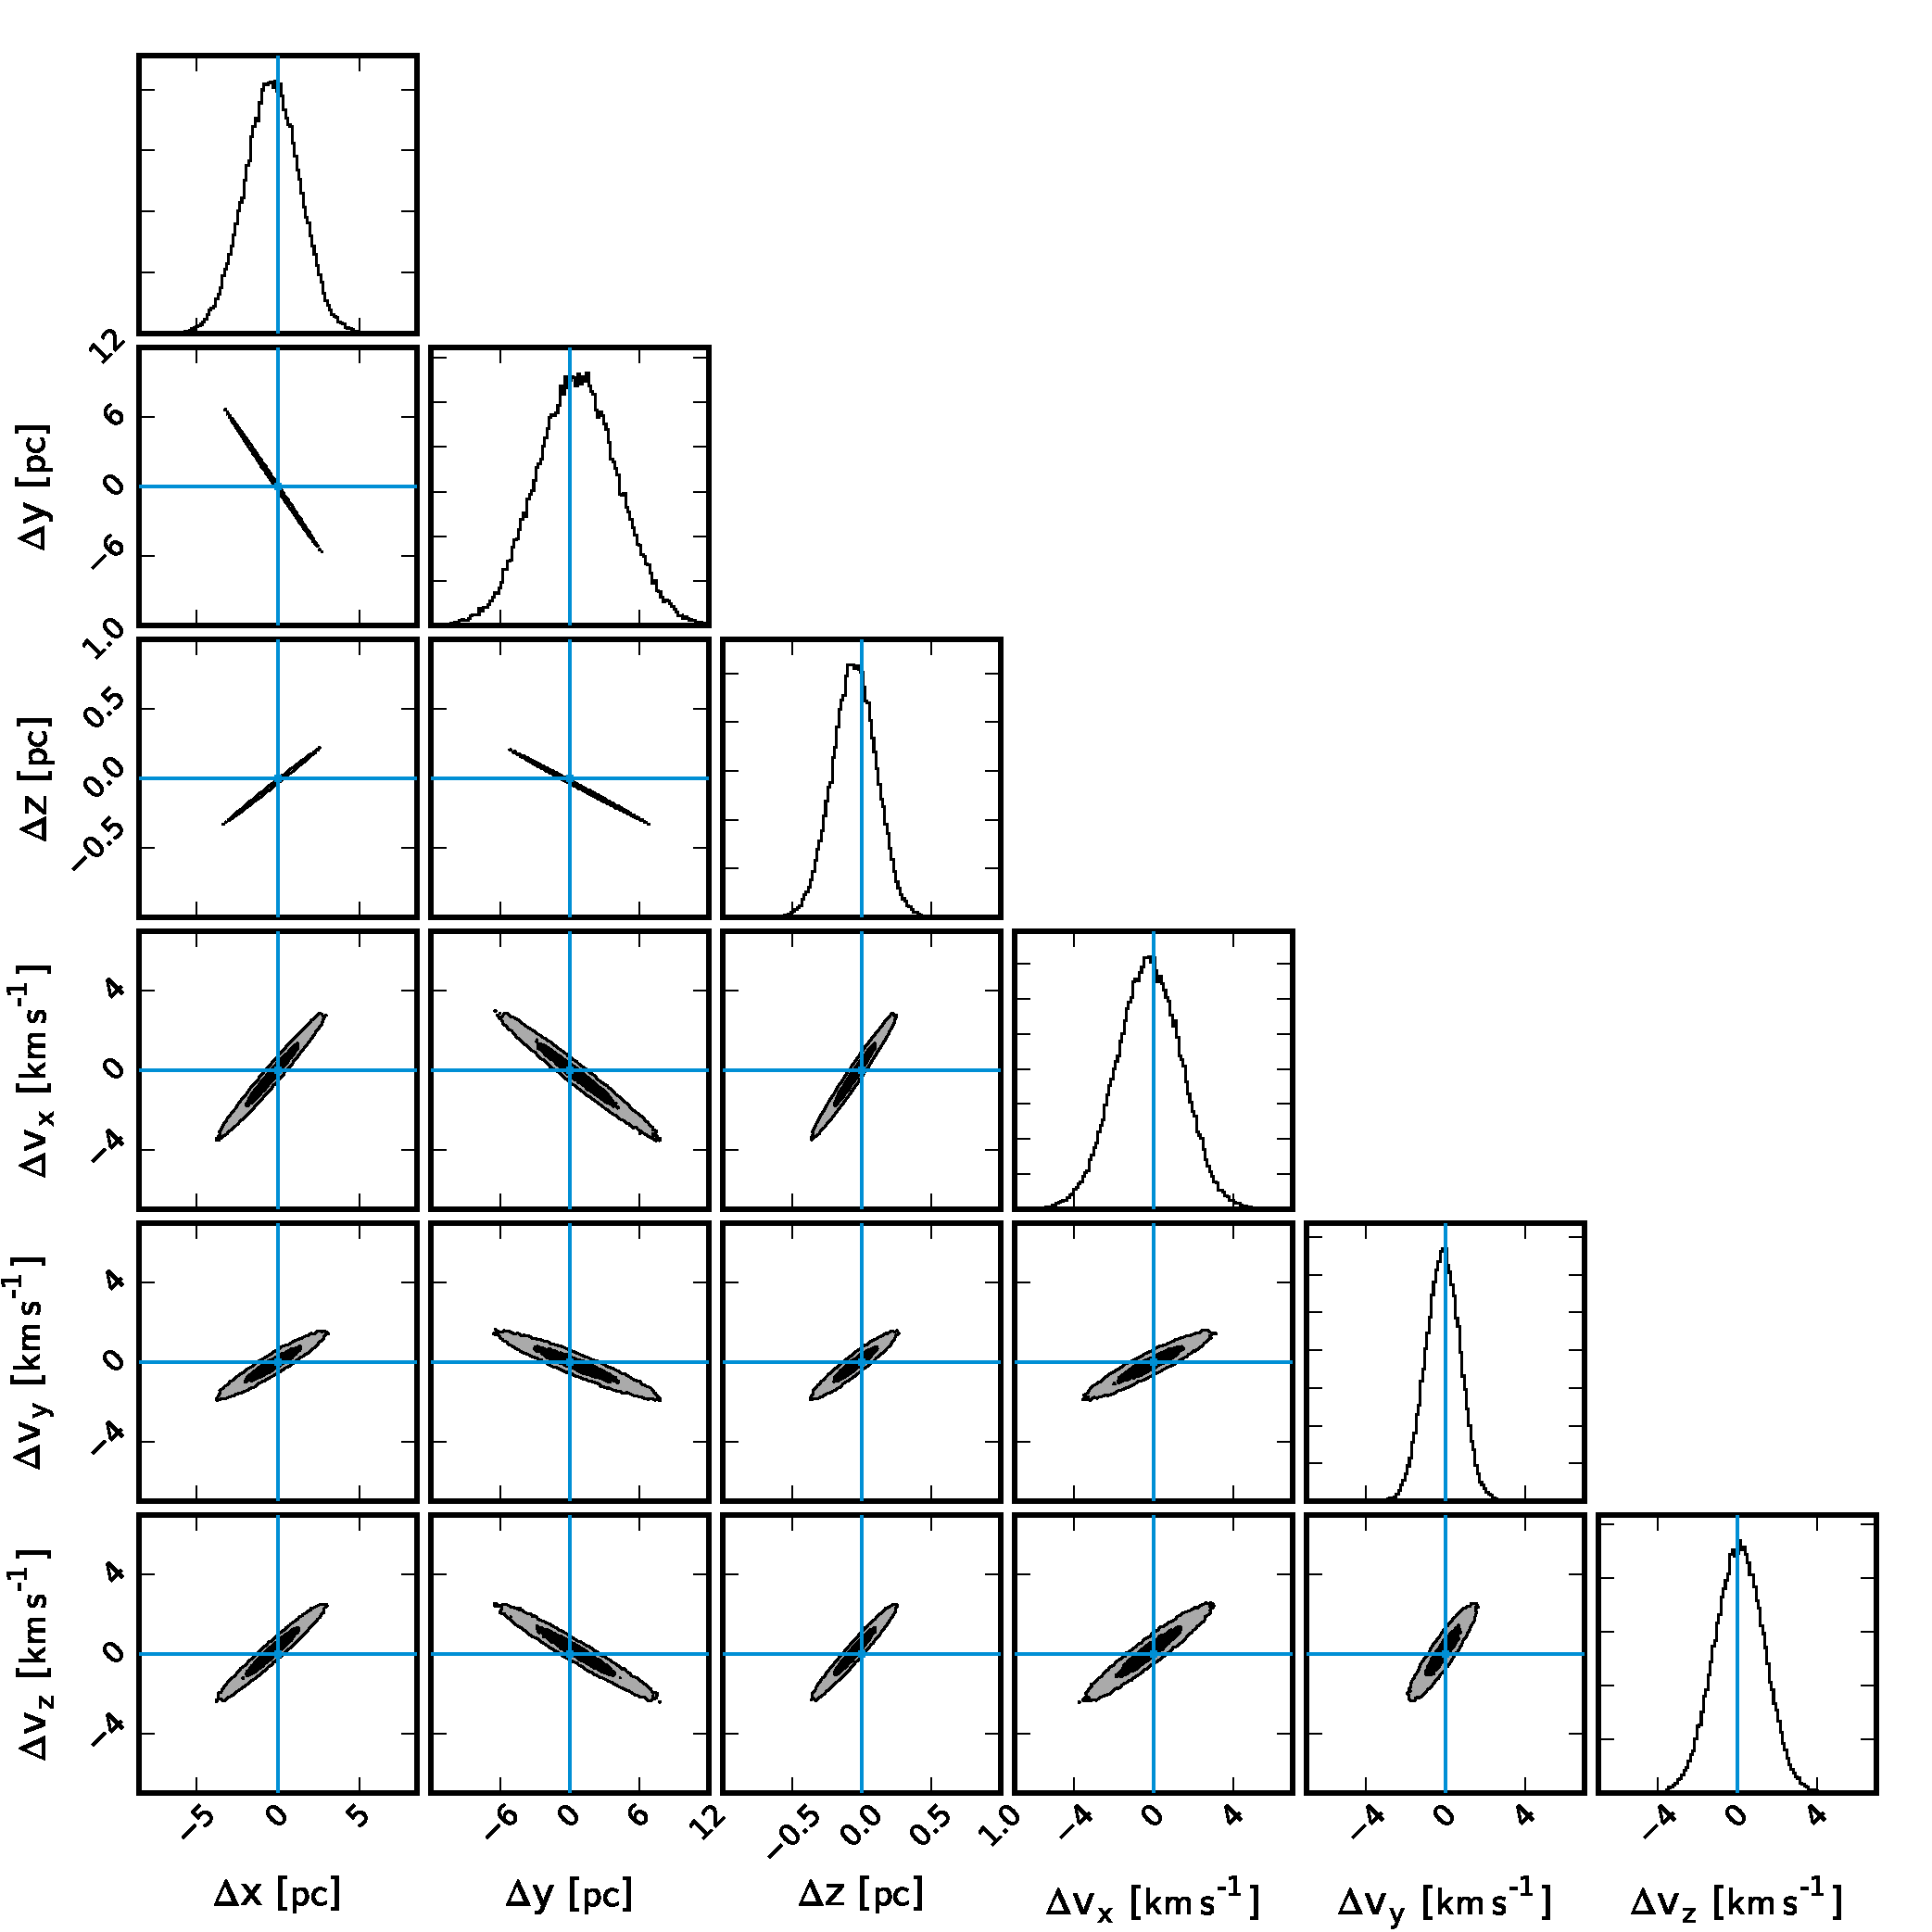
\includegraphics[width=\linewidth]{dx_dv_posterior.pdf}
  \end{center}
  \caption{%
    Differences in posterior samples over Galactocentric phase-space coordinates
    for the two stars \sunanalog\ and \bizarreone.
    \label{fig:dxdv}}
\end{figure}

\figurename~\ref{fig:orbit} shows an orbit computed from the median posterior
sample over 6D phase-space coordinates for \sunanalog\ (black line), integrated
in a Milky Way-like gravitational potential (\cite{Gala:2017}). \todo{APW:
explain}
The Sun's orbit in this same Milky Way model is under-plotted for comparison
(grey line); the orbits of the stars in this pair have large scale-heights
relative to the Sun's orbit despite being young.

\begin{figure}[htbp]
  \begin{center}
    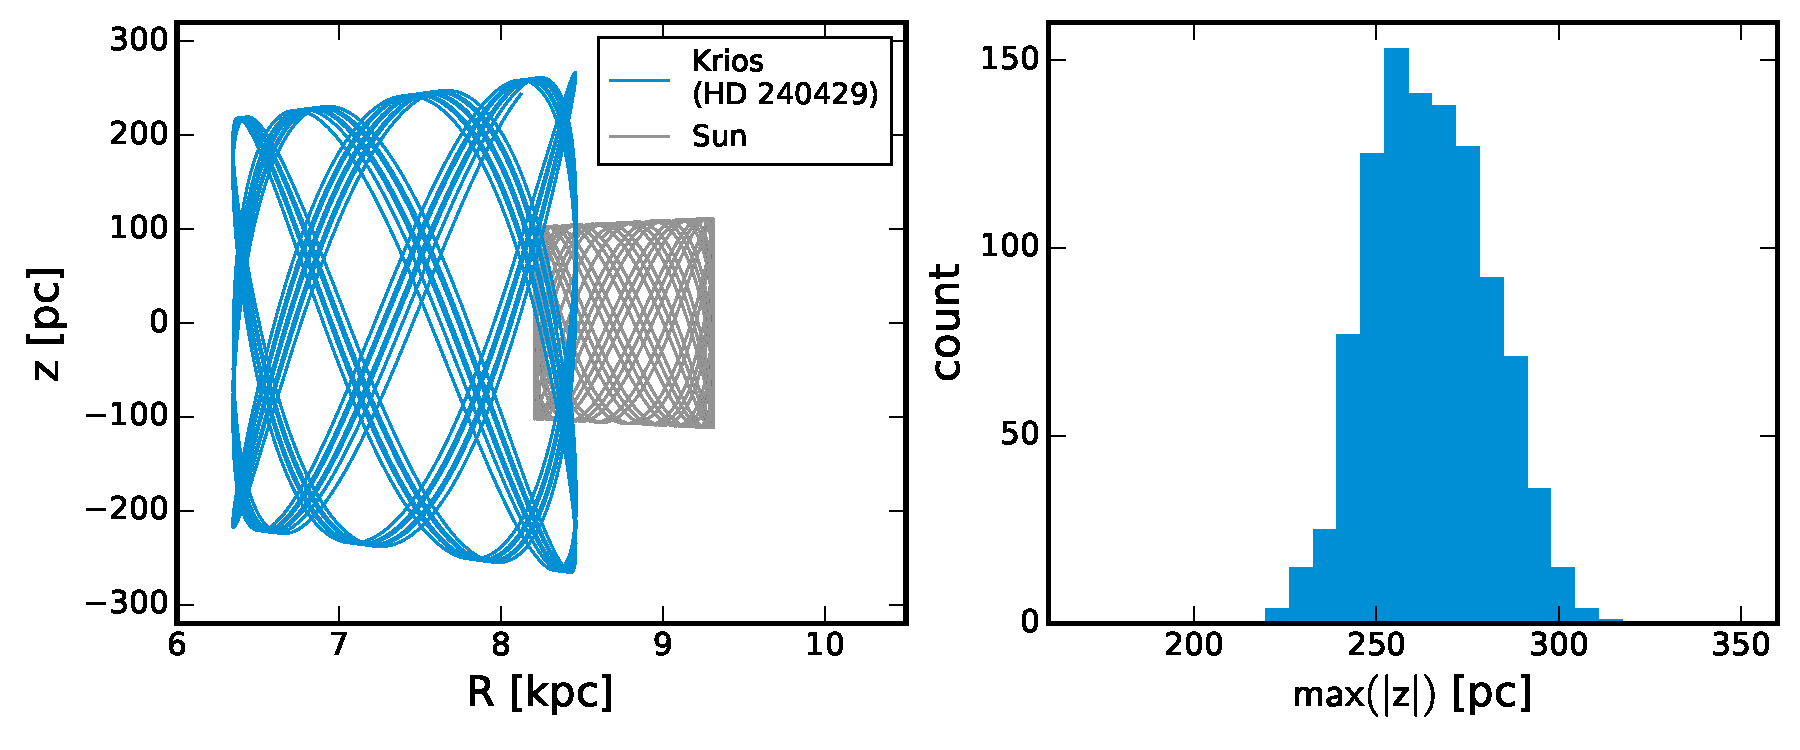
\includegraphics[width=\linewidth]{orbits.pdf}
  \end{center}
  \caption{%
    Galactic orbits computed for \sunanalog\ (black) and the Sun (grey).
    For \sunanalog\, the initial conditions are set to the median posterior
    sample over the inferred 6D phase-space coordinates.
    The orbits are computed by integrating backwards from the present-day
    positions for $2.5~{\rm Gyr}$ with a time-step of $0.5~{\rm Myr}$ using the
    Leapfrog integration scheme implemented in \project{Gala}
    (\citealt{Gala:2017}). \todo{APW: citation...}
\label{fig:orbit}}
\end{figure}

% ----------------
% Horizontal table
% ----------------
% \begin{table*}[htpb]
%   \centering
%   \caption{Astrometric and spectroscopic measurements}
%   \label{tab:t1}
%   \begin{tabular}{cccccccccc}
% \hline\hline
% Name & Sp Type & $T_\mathrm{eff}$ & $\log{g}$ & $v\sin{i}$ & $[\elem{Fe}/\elem{H}]$ & $v_r$ &
% $\varpi$ & $\mu_\alpha^*$ & $\mu_\delta$ \\
% % units
% \hline
% HD 240429 & G2 & 5878 & 4.43 & 1.1 & 0.01 & $-21.2$  & $9.35 \pm 0.24$ & $89.25 \pm 0.66$ & $-29.68 \pm 0.54$\\
% HD 240430 & G0 & 5803 & 4.33 & 2.5 & 0.20 & $-21.2$  & $9.41 \pm 0.25$ & $89.41 \pm 0.69$ & $-30.12 \pm 0.52$\\
% \hline\hline
% \end{tabular}
% \end{table*}

\begin{table*}[htpb]
  \caption{Astrometric and spectroscopic measurements.}
  \label{tab:t2}
  \begin{threeparttable}
  \centering
  \begin{tabular}{ccc}
\hline\hline
Name & HD 240429 & HD 240430 \\
\hline
Sp Type                                   & G2                & G0                \\
$T_\mathrm{eff}$                          & 5878              & 5803              \\
$\log{g}$                                 & 4.43              & 4.33              \\
$v\sin{i}$                                & 1.1               & 2.5               \\
$[\elem{Fe}/\elem{H}]$                    & 0.01              & 0.20              \\
$v_r$                                     & $-21.2$           & $-21.2$           \\
$\varpi$ \footnotemark[1]                 & $9.35 \pm 0.24$   & $9.41 \pm 0.25$   \\
$\mu_\alpha^*$ \footnotemark[1]           & $89.25 \pm 0.66$  & $89.41 \pm 0.69$  \\
$\mu_\delta$ \footnotemark[1]             & $-29.68 \pm 0.54$ & $-30.12 \pm 0.52$ \\
\hline
\multicolumn{3}{c}{$T_c < 1200$~K} \\
\hline
$\elemH{Li}_*$ \footnotemark[2]           & $2.25$            & $2.75$            \\
$\elemH{C}$                               & $0.00$            & $0.09$            \\
$\elemH{N}$                               & $-0.06$           & $-0.01$           \\
$\elemH{O}$                               & $0.01$            & $0.09$            \\
$\elemH{Na}$                              & $-0.06$           & $-0.04$           \\
$\elemH{Mn}$                              & $-0.03$           & $0.00$            \\
\hline
\multicolumn{3}{c}{$T_c > 1200$~K} \\
\hline
$\elemH{Mg}$                              & $0.01$            & $0.19$            \\
$\elemH{Al}$                              & $0.01$            & $0.21$            \\
$\elemH{Si}$                              & $0.00$            & $0.16$            \\
$\elemH{Ca}$                              & $0.02$            & $0.23$            \\
$\elemH{Ti}$                              & $0.02$            & $0.20$            \\
$\elemH{V}$                               & $0.02$            & $0.20$            \\
$\elemH{Cr}$                              & $0.01$            & $0.17$            \\
$\elemH{Fe}$                              & $0.01$            & $0.20$            \\
$\elemH{Ni}$                              & $-0.01$           & $0.21$            \\
$\elemH{Y}$                               & $0.04$            & $0.26$            \\
\hline\hline
\end{tabular}
%
\begin{tablenotes}
  \item All spectroscopic measurements except $\elem{Li}$ are from \citealt{2016ApJS..225...32B}.
  \footnotetext[1]{From \tgas. }
  \footnotetext[2]{Absolute abundance from \todo{CITE}.}
\end{tablenotes}
  \end{threeparttable}
\end{table*}

\todo{Figure: posterior distributions of separation and delta V}

Given their proximity in space and kinematics,
it is generally accepted to assume that the two stars were born coeval
perhaps in a wide binary from the same birth cloud.
Thus, we expect the two stars to have identical metallicities and abundance patterns,
\todo{except for thoese elements like Li...}
Surprisingly, one of the stars, \bizarreone\ is significantly more metal
rich than the other by 0.2~dex ($\approx 60\%$; Figure~\ref{fig:abundances}).
What is more puzzling is that the abundances of this star
shows selective depletion in C, N, O, Na, and Mn.

The abundance of \bizarreone\ is peculiar on its own compared to other disk stars with
similar $[\elem{Fe}/\elem{H}]$.
For a star with $[\elem{Fe}/\elem{H}] \approx 0.2$, we generally expect
$[\elem{Na}/\elem{Fe}] > 0$ and $[\elem{Mn}/\elem{Fe}] > -0.1$
(\citealt{Battistini:2015aa,Bensby:2003aa}) making the abundances of \bizarreone\ ever more unlikely.
We stress that none of the other seven binary pairs examined in \citealt{2016ApJS..225...32B}
show discrepancies in abundances between the stars at this level.
In fact, no strong trend is found in pair for most elements
except N and Y.
For Y, the trend for this pair is opposite of the others in Teff.
Specifically, no difference within pair is found for Mn.
(see figure X in that paper; purple is this pair)

Surface lithium abundance in a sun-like star such as \sunanalog\ decreases with its age
due to mixing induced by convection or rotation which brings lithium
into the interior ($T>2.5 \times 10^{6}$~K)
where it will be destroyed by proton capture burning.
Thus, surface lithium abundance is an indicator of stellar ages.
The $\elem{Li}$ abundance of $2.25$ for \sunanalog\ implies an age of $\lesssim 1$~Gyr
according to the theoretical models tuned to explain the solar lithium abundance
and rotational profile (\citealt{2005Sci...309.2189C}).
The lithium abundance of \bizarreone\ is still higher by $0.5$~dex
showing the largest difference among all measured elements.
This translates to $\sim 500$~Myr difference in age.
Given the overall higher metal abundances and the peculiar abundance patterns in \bizarreone,
it is unclear, however, whether this higher $\elem{Li}$ abundance
means a younger age or something else.
For example, the presence of $\elem{Li}$-rich red giant stars has been attributed
to the engulfment of substellar companions such as gas giant planets or brown dwarfs
which may replenish $\elem{Li}$ (\citealt{Casey:2016aa}).
We come back to the $\elem{Li}$ difference later in our discussion.


\begin{figure}[htpb]
  \centering
  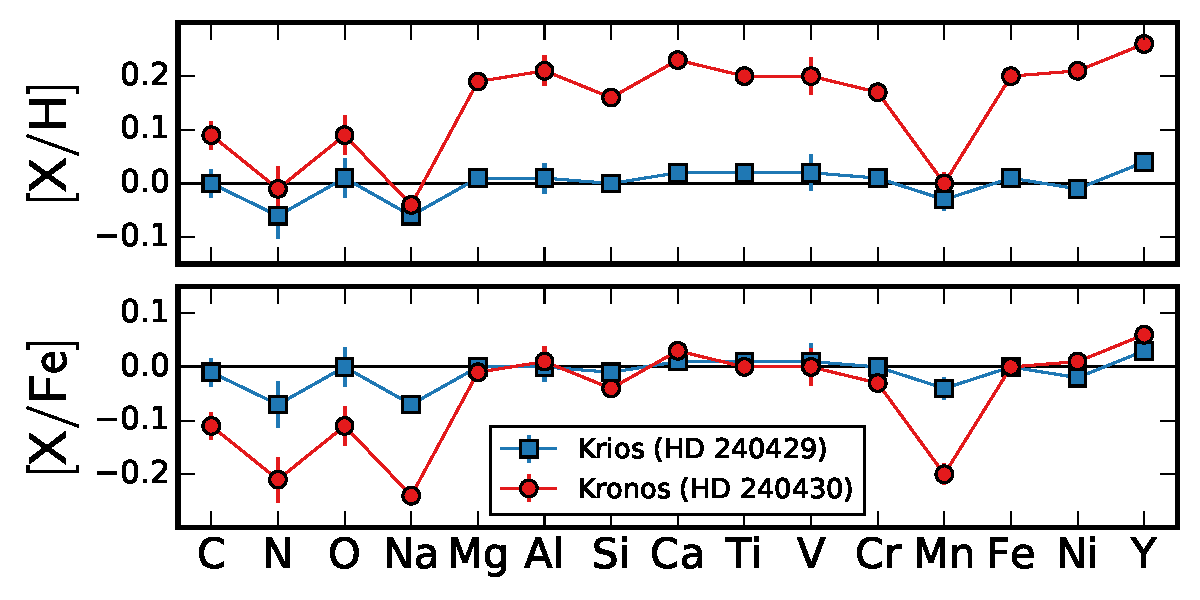
\includegraphics[width=0.9\linewidth]{abundances.pdf}
  \caption{Abundances of the co-moving pair, \sunanalog\ and \bizarreone\.}
  \label{fig:abundances}
\end{figure}

\begin{figure}[htpb]
  \centering
  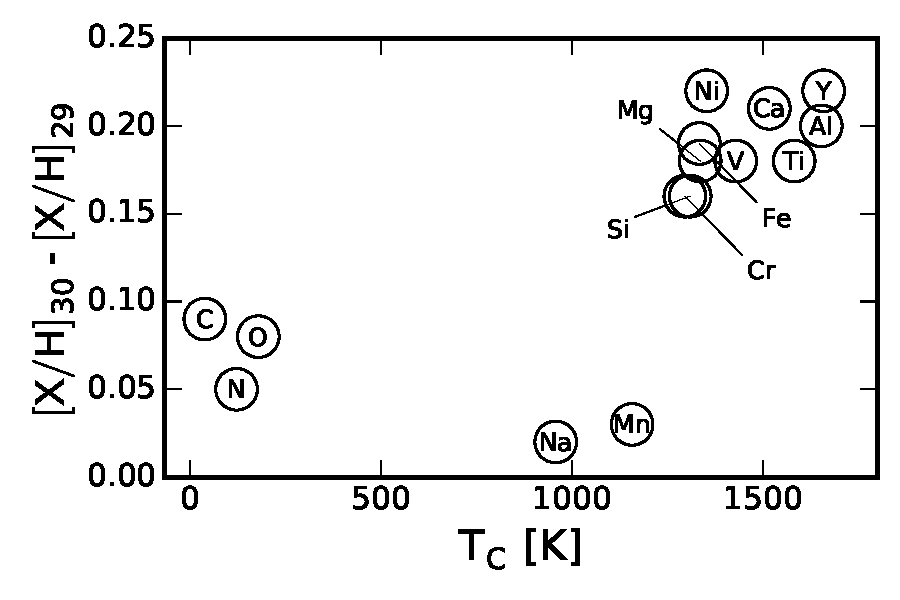
\includegraphics[width=0.9\linewidth]{relabun_tc_XH.pdf}
  \caption{Abundance of \bizarreone\ ($[\mathrm{Fe}/\mathrm{H}] = 0.20$)
    relative to \sunanalog\ ($[\mathrm{Fe}/\mathrm{H}] = 0.01$)
    as a function of condensation temperature of elements (\citealt{2003ApJ...591.1220L}).
  }
  \label{fig:relabun_tc}
\end{figure}

\begin{figure}[htpb]
  \centering
  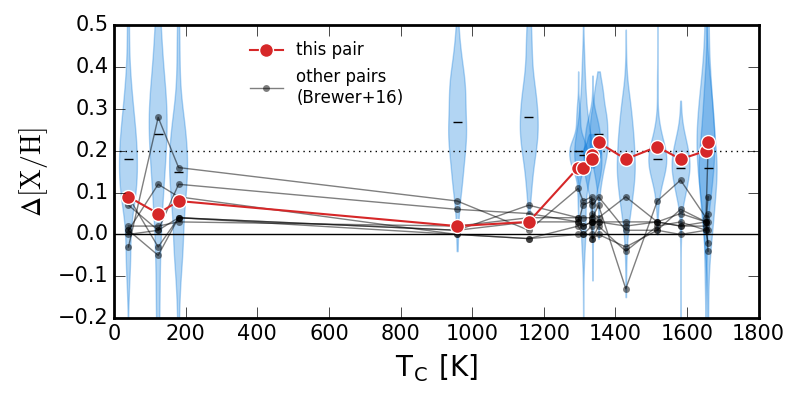
\includegraphics[width=0.9\linewidth]{deltaXH_Tc_violins.png}
  \caption{Difference in abundances of this pair and other binary pairs in
    \citealt{2016ApJS..225...32B}.
    Additionally, we show the distribution of abundance difference
    between stars with similar metallicity difference
    ($\Delta[\elem{Fe}/\elem{H}] \approx 0.2$)
    as violins with medians indicated by black line segments
    by randomly pairing up single stars at two metallicity bins similar to
    the pair of interest.
    The difference is always relative to the lower-$[\elem{Fe}/\elem{H}]$ star.
  }
  \label{fig:deltaXH}
\end{figure}

\section{Discussion}
\label{sec:discussion}

We discuss the possible origins of this pair.
Let us first consider scenarios in which the two stars are not actually born together.

% chance pair
Given that their metallicities and abundance patterns are significantly
different, one may simply conclude that the two stars are not related (coeval)
but they merely happen to be co-moving at such small separation ($\approx 0.6$~pc)
by chance.
The two stars are in the Galactic disk, and assuming certain velocity ellipsoid
at the stars' location, one may compute the probability that a star moving at
the mean velocity of the two stars would have a companion within $\Delta v = XX$~km/s.
...

% binary-single and binary-binary exchange
Two stars unrelated at birth may end up in a binary system via binary-single scattering event
that results in an exchange of binary member.
In order to estimate the rate at which any binary-single
event will produce a wide binary system such as \sunanalog\ and \bizarreone,
we may consider the rate at which this wide binary will scatter with a field star to
result in an exchange reaction.
The cross-section of exchange scattering for a binary with semi-major axis $a$ is
\begin{eqnarray}
  \sigma_\mathrm{ex} = \frac{640}{81} \pi a^{2} \frac{1}{v^6}
\end{eqnarray}
where $v$ is the incoming velocity $v_i$ in units of critical velocity $v_c$ defined as
\begin{eqnarray}
  v_c^2 = G \frac{m_1 m_2 (m_1 + m_2 + m_3)}{m_3 (m_1 + m_2)} \frac{1}{a}
\end{eqnarray}
when $v \gg 1$ using the impulse approximation (\citealt{Hut:1983aa,Hut:1983ab}),
which is appropriate for wide binaries scattering with field (disk) stars.
If we assume that field stars are made of solar mass stars
with constant number density $n=1$~pc$^{-3}$, and the incoming velocity of field stars
is $10$~km\,s$^{-1}$, a lower limit to the velocity dispersions of disk
stars in any direction, the rate of exchange scattering is
\begin{eqnarray}
  n \sigma_\mathrm{ex} v_i = 6.82\times 10^{-8}\,\mathrm{Gyr}^{-1}
  \frac{n}{\mathrm{pc}^3} \frac{\mathrm{pc}}{a} \left(\frac{10~\mathrm{km}\,\mathrm{s}^{-1}}{v_i}\right)^5
\end{eqnarray}
low enough to be negligible.
Because the exchange scattering cross section steeply depends on the incoming velocity
relative to the critical velocity (of the order of orbital velocity of the binary),
the rate of exchange scattering with a star within the same star forming region
may be much larger.
However, even in such scenario, the age difference of $\sim 500$~Myr is too large
for two stars of the same star forming region.

In regions where binarity fraction is high, binary-binary scattering may be more important
than binary-single scattering (\todo{CITE})


%Two factors that make this even more unlikely are that both stars are very young given their large Li,
%and that if the pair is a result of scattering, one expect to end up with typical stars of the field,
%not HD30 with anomalous abundance patterns.


None of the above scenarios is satisfactory as it offers no
insight on the peculiarity in abundances of HD 30 (see \sectionname~{\ref{sec:data}).

The unlikeliness of the above possibilities naturally leads us to
consider the alternative.
What can selectively enrich XX elements in one of the two stars that are born together?

% inhomogeneity in star formation
It may be that the two stars are born at the same time from the same cloud, but
there is inhomogeneity within the cloud.
However, there is already ample amount of evidence against such scenario.
First, none of the other seven similar wide binaries examined in \citealt{2016ApJS..225...32B}
show the same level differences in abundances although there is generally
a larger spread in $\elem{C}$, $\elem{N}$ and $\elem{O}$, and some pairs show
a large as $\approx 0.15$~dex difference in particular elements.
The median and maximum \feh\ difference between component stars in the other seven pairs
is $0.02$~dex and $0.09$~dex, respectively.
This is consistent with the findings of \citealt{Desidera:2004aa} who examined 23 wide bianries
of late F to K dwarfs, and found most pairs show difference in \feh\ less than $0.02$~dex
and none larger than $0.07$~dex.

% summarize other pair studies in detailed chemical abundance here

% rocky planets (or the like) engulfment
Yet another possibility is that the more metal-rich of the two stars
was recently? bombarded by something that selectively removed the depleted elements but not the others.

estimate: 10 earth mass

Present the relative abundance figure here

Change in stellar abundance due to ingestion of planets has been considered
for similar bright star pairs HD XX/XX (Mack) and HD XX/XX(Mack).


% Concluding remakrs


\bibliography{ref}



\end{document}
